\chapter{Results}

Um die Ergebnisse richtig einordnen zu können stellen wir an dieser stelle kurz die Ausgangsdaten dar.

Die relativen Produktionsquantile die zum exportieren der anderen Zeitreihenabschnitte gedient haben stellen sich wie folgt dar:

\begin{figure}[!h]
	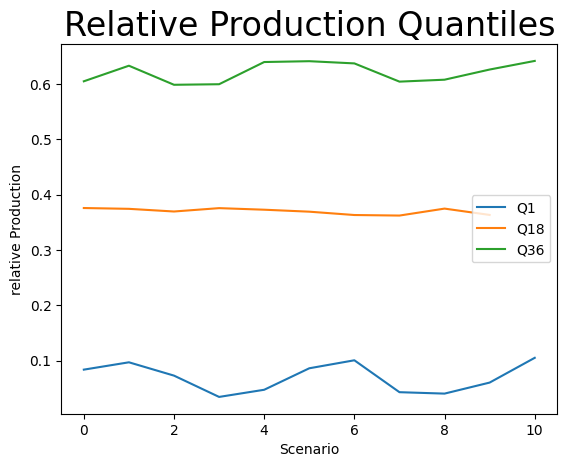
\includegraphics[width=0.7\linewidth]{pictures/results/relativeProduktionQuantils.png}
	\caption{Relative Production Quantiles}
	\label{fig:Relative Production Quantiles}
\end{figure}

Die daraus Resultierenden Zeitreihen für aktivierte Regelarbeit und deren Preise stellen sich dann wie folgt dar:

Für den selben Zeitabschnitt lässt sich der DA Markt wie folgt zusammenfassen:


Außerdem stellt sich der entsprechende RL Markt wie folgt dar:

Dabei zeigt sich das mit steigender Marktdurchdringung der volatilen Energieproduktionsquellen vor allem die Menge an aktivierter Negativer
RegelArbeit steigt während die nachfrage nach positiver regelarbeit fällt.

Ein ähnliches Bild zeigt sich bei den Grenzpreisen für die aktivierte Regelarbeit. wärend die Preise für negative Regelarbeit mit
zunehmenden Anteil an volatilen Produzenten zunimmt, gehen die Preise für die positive Regelarbeit zurück.

Bemerkenswert ist allerdings das sehr hohe Ausreißer in den Zeitreihen für die Grenzpreise der  positiven Regelarbeit bei mittlere und geringer
Marktdurchdringung durch volatile Produzenten zu sehen ist.
--> das liegt vermutlich daran das in den Szenarien wo man mögliche große schwankungen erwartet darauf vorbeiretet ist.
--> Aber in den Szenarien in denen die mehrheit der Anbieter nicht damit rechnet scheint eine unerwartet hohe Nachfrage
--> einen preisschock aus zu lösen.

Die medianen \todo{eventuell nochmal erklärung in data abschnitt wieso das hier die medianen sind} KApazitätspreise für Regelarbeit peaken
sowohl für die negative als auch für die positive im mittleren Szenario. In den Daten des ersten Quantils sind die sie für die negative Regelleistung
vergleichbar mit denen des 36. Quantils. Für die positive Regelleistung hebt sich das 36. Quantil von 1. Quantil vor allem im späten Tagesverlauf ab.

--> es scheint so als würden viele anbieter damit rechnen am folgenden Tag Regelarbeit zu liefern. Dabei hantiert der Regelleistungspreis
--> als eine Art mitnahme preis was zur folge hat das das Angebot noch stärker steigt als die Nachfrage und so sinkende Regelleistungspreise zur folge hat.

Auf Grundlage dieser Zeitreihen hat das Model folgende Daten ermittelt.

Die Strategie für die Gebotspreise für den Kapazitätsmarkt bewegt sich über alle Szenarien hinweg knapp unterhalb des erwarteten Grenzpreises.
\todo{grafik hierfür einblenden  .. !! eher wichtig !!}

Zu sehen ist das die Bereitstellung der negativen RegelArbeit
in den niedrigen und mittleren Szenarien früher erfolgt wenn beide Regelleistungsgebot angenommen wurden [Figure \ref{fig:Negative Balance Energy - Q1}, \ref{fig:Negative Balance Energy - Q18}].
--> verpflichtungen und insgesamt regelmäßigere ladekurve wärend in den höheren Preisszenarien mehr wert
--> darauf gelegt wird wirklich die preisspitzen möglichst optimal mit nehmen zu können.
--> ob das in der realität oder perfektes wissen innerhalb des szenarios so erfolgen kann ist fraglich
In den Szenarien mit den hoher produktiver volatilität ist diese Verschiebung nicht fest zu stellen [Figure \ref{fig:Negative Balance Energy - Q36}]


Wärend sich die Gebotsmengen zur postiven Regelarbeit, je nach Bezuschlagung am Regelleistungsmarkt,
kaum in dem niedrigen und mittleren Szenario voneinander unterscheiden. sind deutlichere Unterschiede
im Szenario mit hoher volatiler Produktion zu erkennen. Auch hier erfolgt eine frühere Bereitstellung
der Arbeit bei stärkeren Restriktionen durch die Bezugschlagung am Regelleistungsmarkt.



Zum Verständnis
\begin{enumerate}
	\item Restricted: B $\rightarrow$ accepted RL in \& out
	\item Restricted: O $\rightarrow$ accepted RL out \& dclined in
	\item Restricted: I $\rightarrow$ accepted RL in \& dclined out
	\item Restricted: N $\rightarrow$ declined RL in \& out
\end{enumerate}

Die Ergebnisse zeigen eine relativ stetiges Gebotsverhalten am Kapazitätsmarkt über alle Szenarien hinweg.

-->Es wird gerade soviel Geboten
das der Batteriespeicher immer sicher die Restriktionen erfüllen kann ohne all zu sehr den Regelarbeitsmarkt zu beeinflussen.

\begin{figure}[!h]
	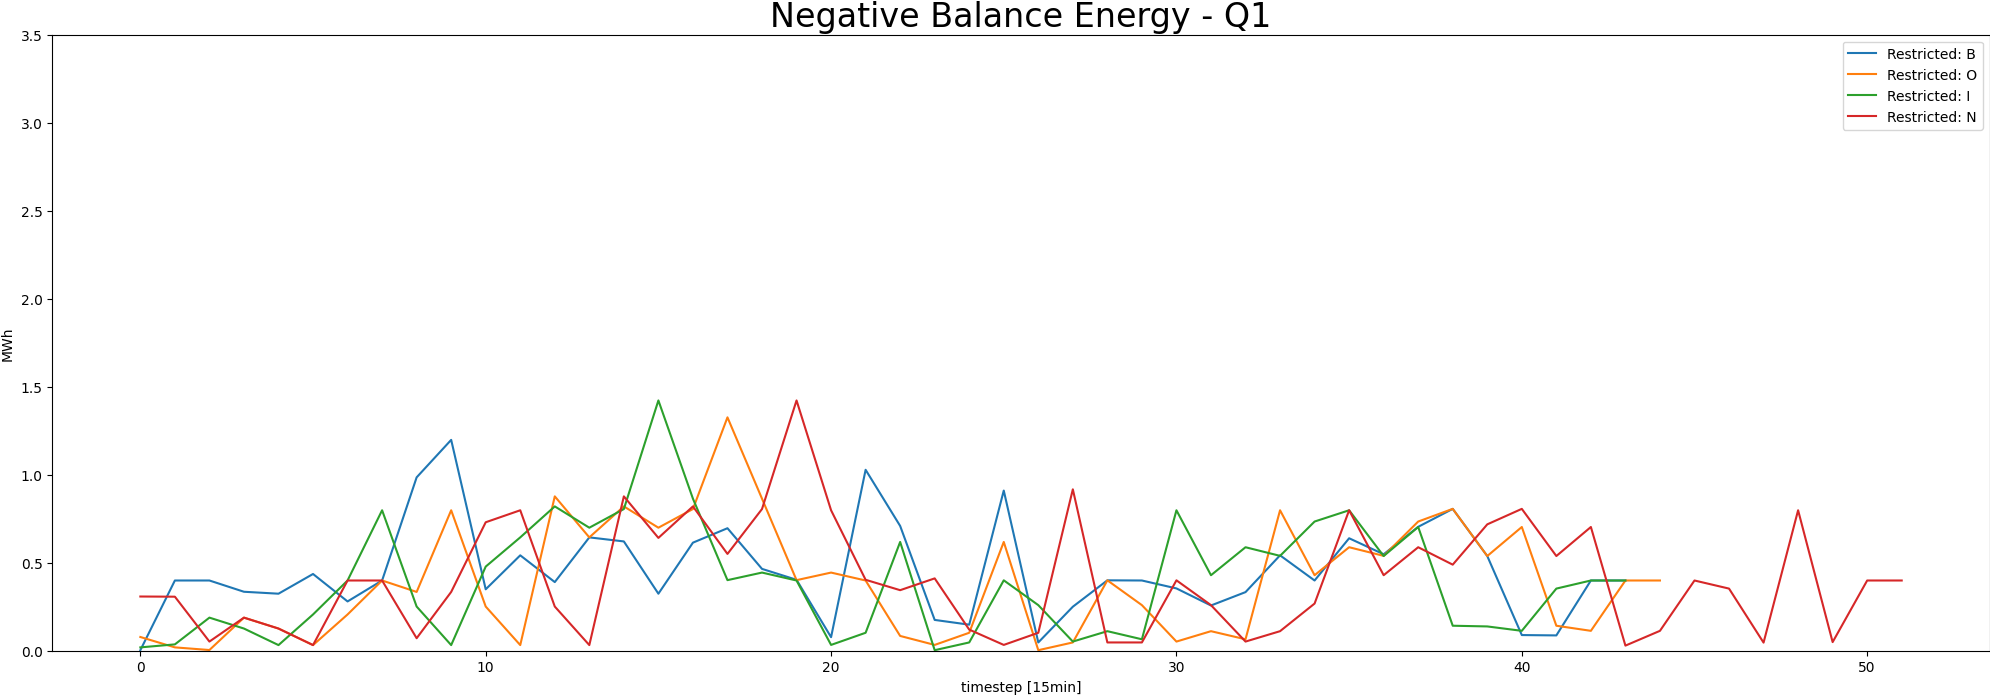
\includegraphics[width=1\linewidth]{pictures/results/Negative Balance Energy - Q1.png}
	\caption{Negative Balance Energy - Q1}
	\label{fig:Negative Balance Energy - Q1}
\end{figure}

\begin{figure}[!h]
	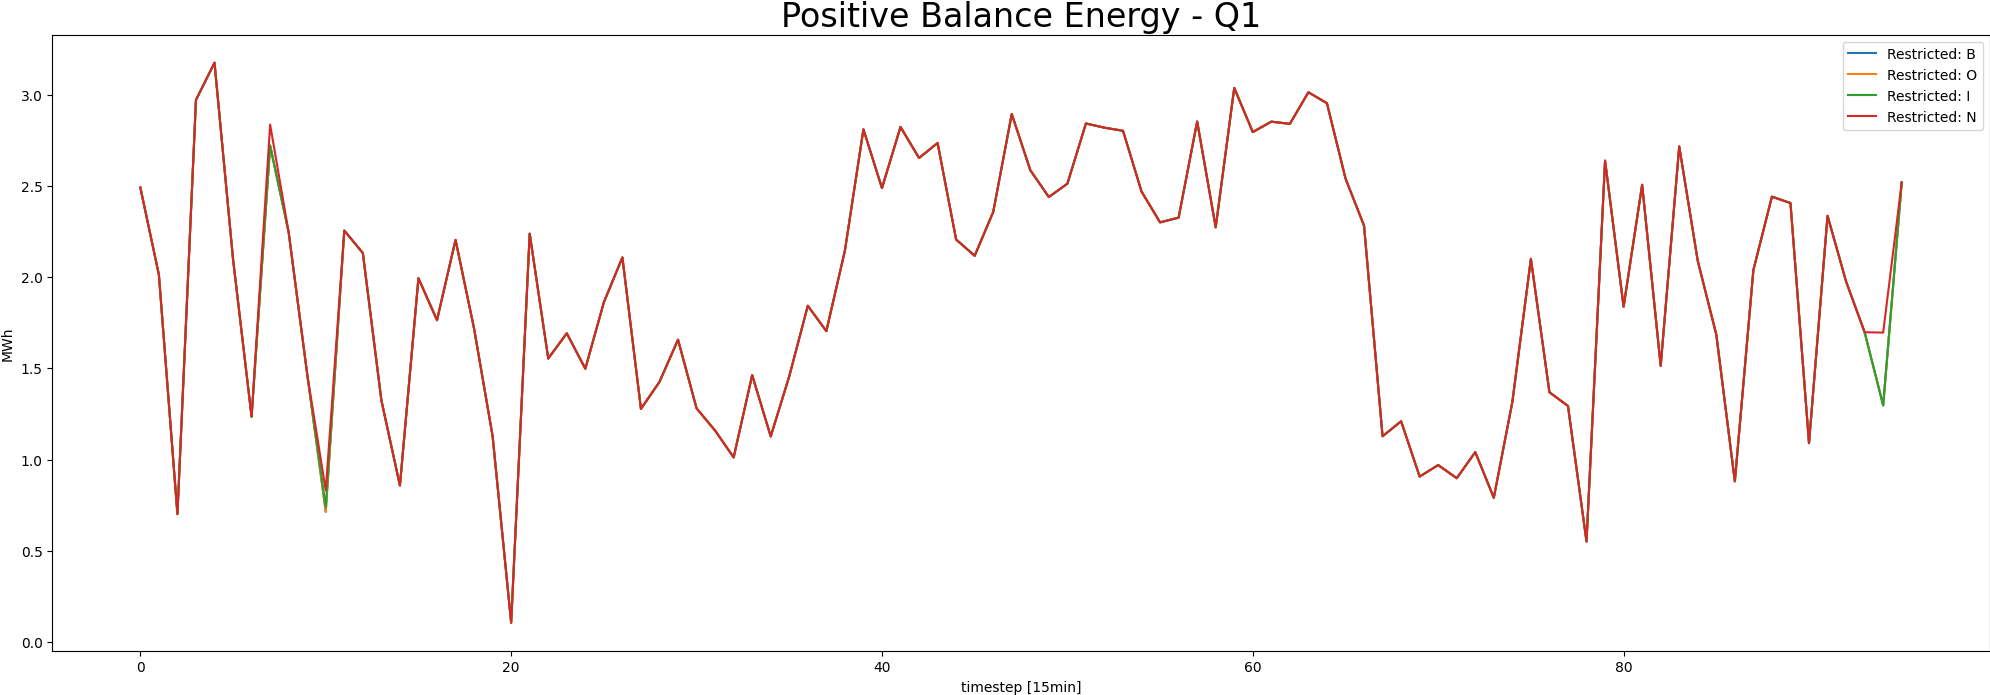
\includegraphics[width=1\linewidth]{pictures/results/Positive Balance Energy - Q1.png}
	\caption{Negative Balance Energy - Q1}
	\label{fig:Negative Balance Energy - Q1}
\end{figure}



\begin{figure}[!h]
	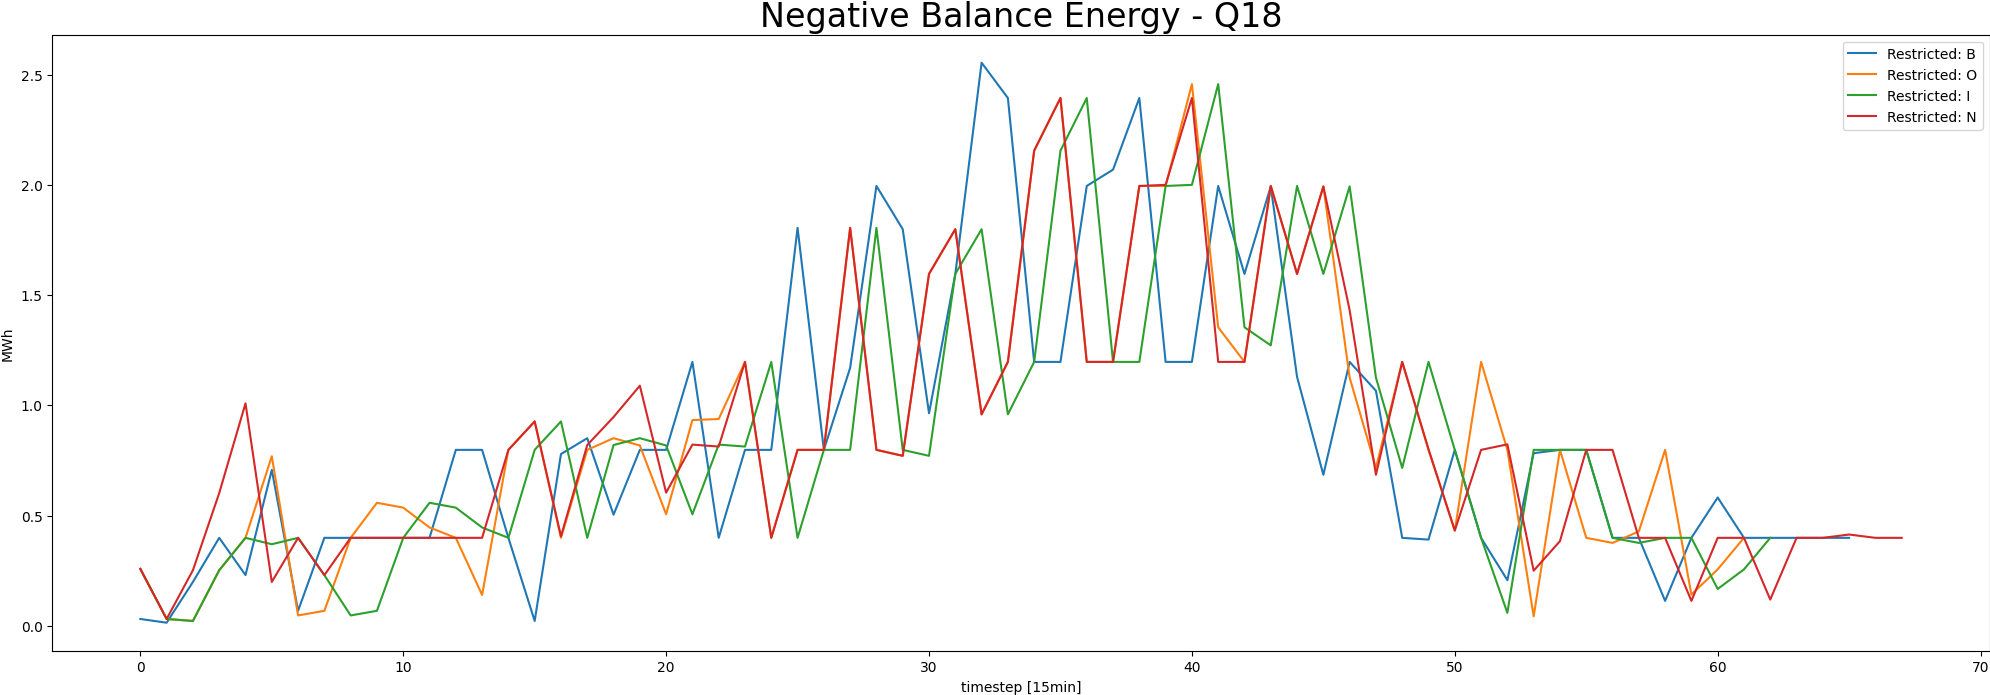
\includegraphics[width=1\linewidth]{pictures/results/Negative Balance Energy - Q18.png}
	\caption{Negative Balance Energy - Q18}
	\label{fig:Negative Balance Energy - Q18}
\end{figure}

\begin{figure}[!h]
	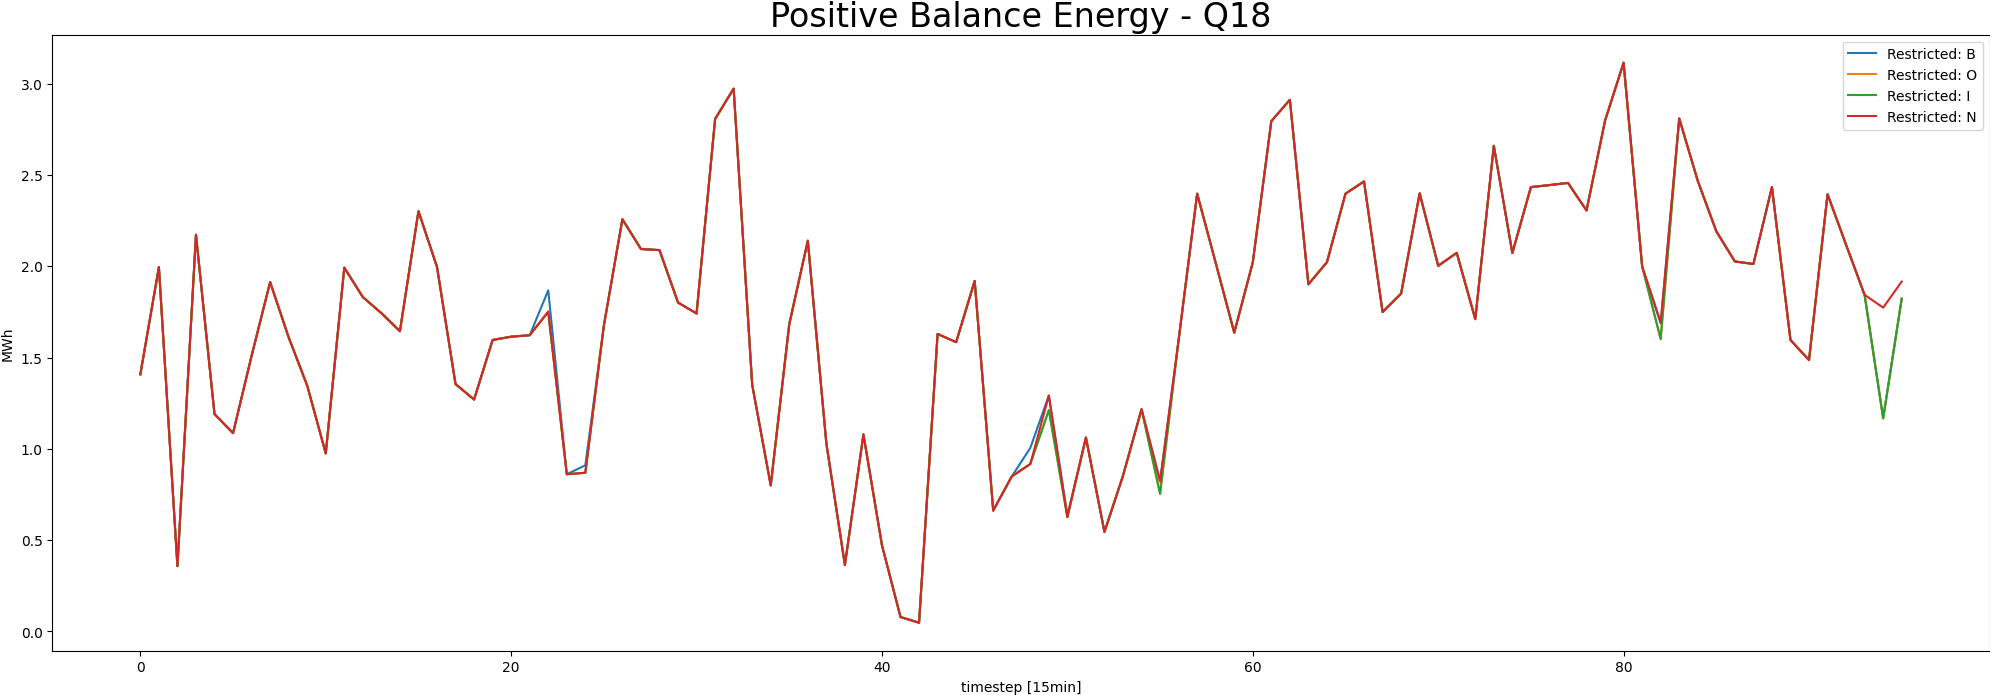
\includegraphics[width=1\linewidth]{pictures/results/Positive Balance Energy - Q18.png}
	\caption{Negative Balance Energy - Q18}
	\label{fig:Negative Balance Energy - Q18}
\end{figure}




\begin{figure}[!h]
	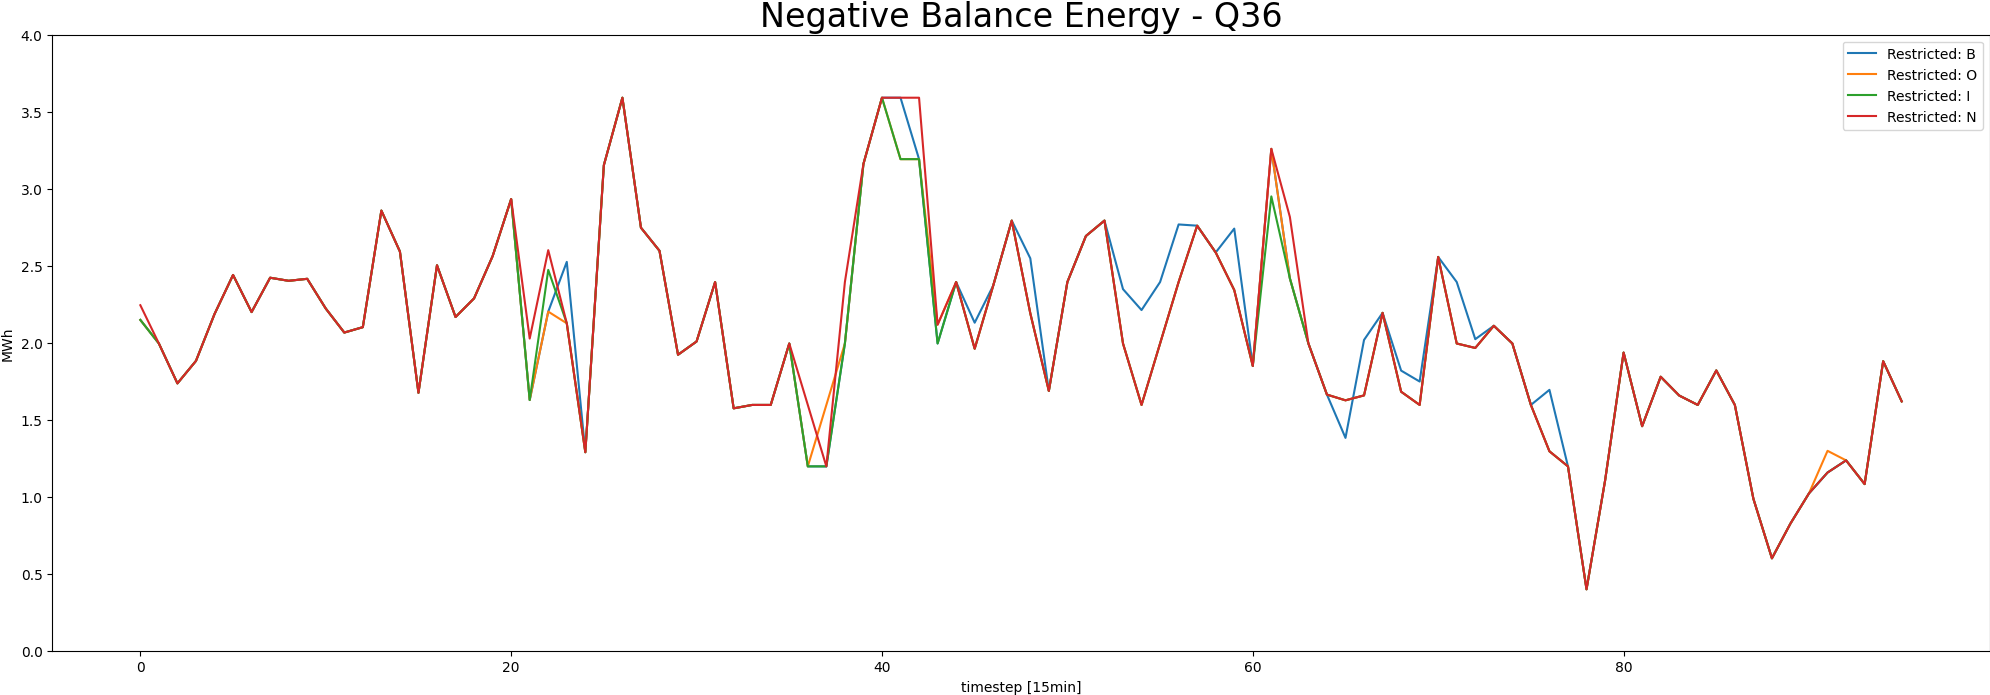
\includegraphics[width=1\linewidth]{pictures/results/Negative Balance Energy - Q36.png}
	\caption{Negative Balance Energy - Q36}
	\label{fig:Negative Balance Energy - Q36}
\end{figure}

\begin{figure}[!h]
	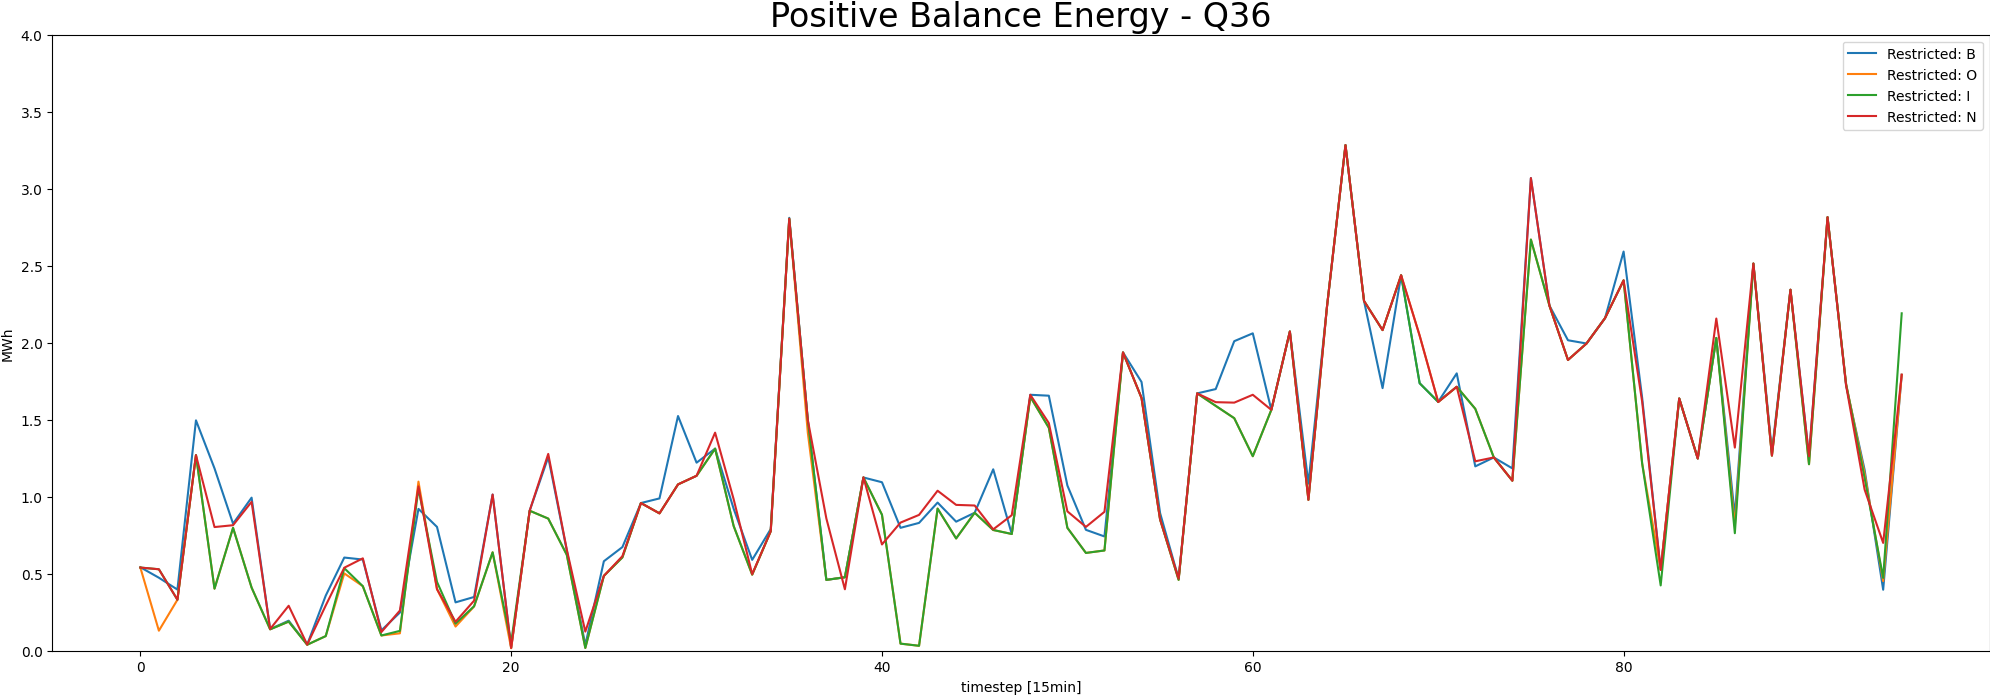
\includegraphics[width=1\linewidth]{pictures/results/Positive Balance Energy - Q36.png}
	\caption{Negative Balance Energy - Q36}
	\label{fig:Negative Balance Energy - Q36}
\end{figure}


